\section{Décentralisé vs Centralisé}
\subsection{Principe de base d'un VCS}
\begin{frame}{Principe de base d'un VCS}
  Gérer le mécanisme lecture-fusion-écriture
  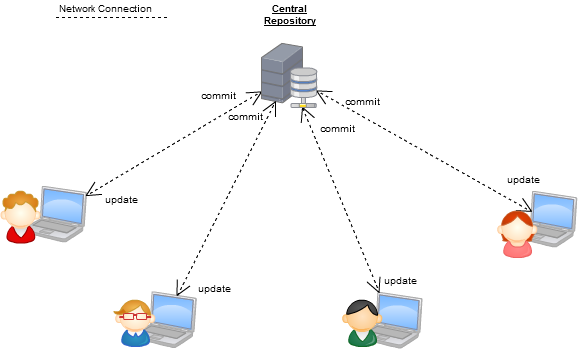
\includegraphics[width=\textwidth]{./diapo1.png}
\end{frame}

\subsection{Gestionnaire de versions centralisé CVCS}
\begin{frame}{Gestionnaire de versions centralisé CVCS}
  \begin{columns}[T]

    \begin{column}{.6\textwidth}
      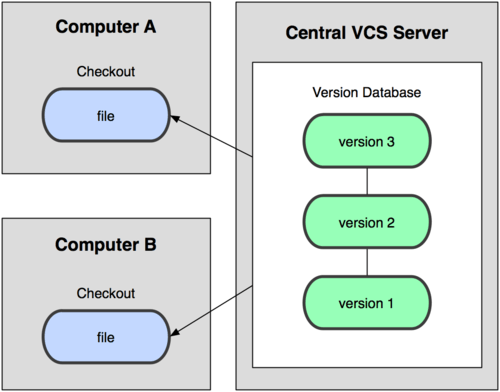
\includegraphics[width=\textwidth]{./CVCS.png}
    \end{column}

    \begin{column}{.4\textwidth}
      \begin{itemize}
        \item{Un seul dépôt de référence (serveur)}
        \item{Les utilisateurs travaillent sur une copie}
      \end{itemize}
    \end{column}

  \end{columns}
\end{frame}

\begin{frame}{Gestionnaire de versions centralisé CVCS}
  Qualités:
  \begin{itemize}
    \item{technologie éprouvée}
    \item{largement disponible}
    \item{sécurisé}
  \end{itemize}

  Défauts:
  \begin{itemize}
    \item{échange entre les dépôts impossible}
    \item{échange entre les copies locales impossible}
    \item{travail hors connexion impossible}
    \item{dépendant du serveur}
  \end{itemize}
\end{frame}

\subsection{Présentation SVN}
\begin{frame}{Présentation SVN}
  Serveur centralisé et unique:
  \begin{itemize}
      \item{les fichiers de reférences (le dépôt ou repository)}
      \item{un logiciel serveur SVN tournant en tâche de fond}
  \end{itemize}

  Postes clients:
  \begin{itemize}
      \item{copie locale du repo, éventuellement modifié}
      \item{logiciel client permettant la synchronisation manuelle et/ou
            automatisée entre chaque client et le serveur de ref}
  \end{itemize}
  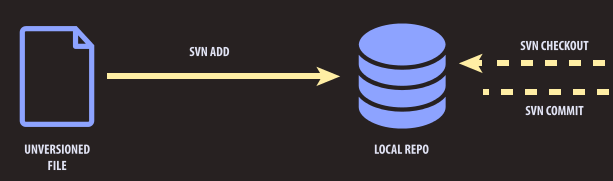
\includegraphics[width=\textwidth]{./svn1.png}
\end{frame}

\subsection{Gestionnaire de versions décentralisé DVCS}
\begin{frame}{Gestionnaire de versions décentralisé DVCS}
  \begin{columns}[T]

    \begin{column}{.6\textwidth}
      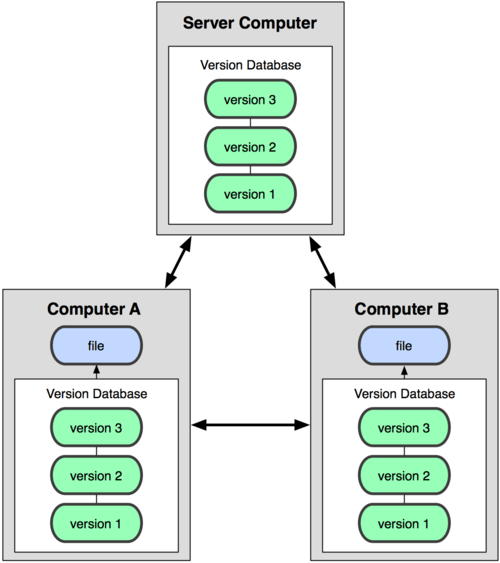
\includegraphics[width=\textwidth]{./DVCS.png}
    \end{column}

    \begin{column}{.4\textwidth}
      \begin{itemize}
        \item{Dépôt propre à chaque développeur}
        \item{Copie propre à chaque développeur}
      \end{itemize}
    \end{column}

  \end{columns}
\end{frame}

\begin{frame}{Gestionnaire de versions décentralisé DVCS}
  Qualités:
  \begin{itemize}
    \item{communication possible entre les dépôts}
    \item{possibilité de mettre en place un dépôt central (serveur)}
    \item{travail hors connexion possible}
    \item{indépendant du serveur}
    \item{gestion des branches}
    \item{gestion des merges}
  \end{itemize}

  Défauts:
  \begin{itemize}
    \item{complexité (Git)}
  \end{itemize}
\end{frame}
